\documentclass[11pt,a4paper]{article}
\usepackage[margin=2.4cm]{geometry}
\usepackage{fontspec}
\usepackage{booktabs}
\usepackage{amsmath}
\usepackage{xcolor}
\usepackage{tikz}
\usetikzlibrary{positioning,arrows.meta,shapes.misc,calc}
\usepackage{enumitem}
\usepackage{hyperref}
\usepackage{microtype}
\usepackage{needspace}
\setlength{\parskip}{6pt}
\setlength{\parindent}{0pt}
\definecolor{pink}{HTML}{CF1A5C}
\definecolor{blue}{HTML}{2D6BB5}
\definecolor{grey}{HTML}{7D8893}
\definecolor{ink}{HTML}{101820}
\hypersetup{colorlinks=true,linkcolor=blue,urlcolor=blue}

\title{\Huge Teaching a Computer to Point at the Right Part of a Drawing\\[6pt]
\Large The ``semantic prior'' experiment, explained in simple words}
\author{SVG Patch Lab}
\date{10 September 2026}

\begin{document}
\maketitle

\section*{The problem, in one picture}

An SVG is a drawing made of lines. Each line has a name: \texttt{n1}, \texttt{n2}, \texttt{n3}, and so on.
Someone types an instruction like \emph{``Change the camera lens to red.''}
The computer has to answer one question: \textbf{which line is the lens?}

\begin{center}
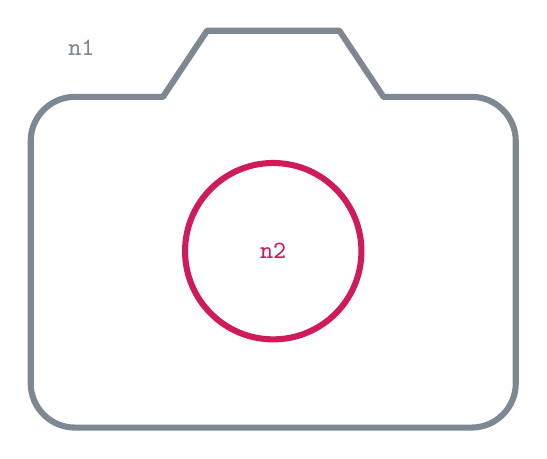
\begin{tikzpicture}[line width=2.2pt, line cap=round, line join=round, scale=0.28]
  % camera body (n1), drawn in grey
  \draw[grey] (23,5) .. controls (23,3.9) and (22.1,3) .. (21,3) -- (3,3) .. controls (1.9,3) and (1,3.9) .. (1,5) -- (1,16) .. controls (1,17.1) and (1.9,18) .. (3,18) -- (7,18) -- (9,21) -- (15,21) -- (17,18) -- (21,18) .. controls (22.1,18) and (23,17.1) .. (23,16) -- cycle;
  % lens (n2), in pink
  \draw[pink] (12,11) circle (4);
  \node[grey, font=\ttfamily\small] at (3.3,20.2) {n1};
  \node[pink, font=\ttfamily\small] at (12,11) {n2};
\end{tikzpicture}

\small The camera icon from the Feather set. The body is \texttt{n1}; the lens is \texttt{n2}.
\end{center}

If the computer points at the right line, we can change its colour safely and nothing else in the drawing is touched.
If it points at the wrong line, the drawing breaks.
So the whole game is \textbf{pointing at the right line}.

\section*{Why we did this experiment}

Before today, our pointing brain got the right answer on only \textbf{22 out of 100} new drawings.
When we looked at the mistakes, \textbf{48 of them were ``wrong part''} mistakes: it pointed at the camera body when asked for the lens, or at the battery when asked for the lightning bolt.

Why? The old brain was trained only on \emph{made-up practice drawings} where the instructions used simple words like ``the red circle on the left''.
It had never seen the words \emph{lens}, \emph{lightning bolt}, \emph{bell}, or \emph{hull}.
When it heard a word it did not know, it just guessed the biggest line.

So the idea was simple: \textbf{add a helper that already knows what things look like.}

\section*{The data we used}

There are three piles of drawings. Keeping them apart is the most important rule.

\begin{description}[leftmargin=1.6em, style=nextline]
  \item[1. Practice drawings (made up by a program).] Thousands of simple scenes with instructions like ``the small blue square''. The old brain learned from these. Nothing new was trained today, so today they were only used to make the old brain's scores.
  \item[2. The old test (80 drawings).] Real icons from two collections called Hicon and Streetmix, with real instructions from a public dataset (VectorEdits). Their right answers were worked out automatically by comparing the before and after drawings, so they are a bit rough. We used this pile like a \emph{practice exam}: to choose one knob (see below) and nothing else.
  \item[3. The real test (100 instructions on 50 icons).] Icons from two collections called Feather and Tabler that nobody in this project had used before. Two instructions were written for each icon, for example ``Change the clock hands to red''. Every right answer was checked by eye in the drawing. 45 of the 100 answers need \emph{more than one line} (for example both wheels of a truck). This pile is \textbf{sealed}: a fingerprint (a hash) of the file is stored, and the program refuses to run if the file changes. Nobody tunes anything on it. Today was the third time it was ever scored.
\end{description}

\section*{The pieces of the machine}

\subsection*{The old brain (a small neural network)}

The old brain is a tiny network (a ``no-edge MLP''). For each line in the drawing it looks at numbers: how big the line is, where it sits, what colour it has, what kind of shape it is.
It reads the instruction with a cheap trick called \emph{hashing}, which turns words into numbers without understanding them.
It gives every line a score from 0 to 1, and it has a second little part, the \textbf{count head}, that guesses \emph{how many} lines to pick.
Then it sorts the lines by score and picks the top ones.
It is frozen: we did not change it at all today.

\subsection*{The new helper (SigLIP 2)}

SigLIP 2 is a big model that Google trained on hundreds of millions of pictures with captions.
It can look at a picture and a sentence and say \emph{how well they match}.
We did not train it either. We just use it.

For each line in a drawing we make three small pictures:
\begin{itemize}[leftmargin=1.6em]
  \item the line \textbf{alone} on a white background,
  \item a \textbf{zoomed-in} view with that line highlighted in pink,
  \item the \textbf{whole icon} with that line highlighted in pink.
\end{itemize}
We show all three pictures and the words that name the part (``the camera lens'') to SigLIP.
It gives a matching score for each line. The three pictures are mixed with fixed weights (half, a third, and a fifth) that were chosen in an earlier experiment and left alone.

\subsection*{Mixing the two, with one knob}

Now every line has two scores: one from the old brain and one from the helper.
We add them together with one knob called $\alpha$ (alpha) between 0 and 1:

\[
\text{final score} \;=\; (1-\alpha)\times(\text{old brain's score}) \;+\; \alpha\times(\text{helper's score}).
\]

$\alpha = 0$ means ``only the old brain''. $\alpha = 1$ means ``only the helper''.
(The two scores live on different scales, so under the hood the old brain's score is turned into a \emph{logit} and the helper's is multiplied by SigLIP's own built-in scale of about 113. That is just so they can be added fairly.)

\textbf{How we chose the knob.} We tried eleven values of $\alpha$ on the \emph{practice exam} (the 80 old drawings) and wrote down, \emph{before} looking, the rule for picking the winner: the value that gets the most drawings exactly right.
$\alpha = 0$ gave 41 out of 80, exactly what the old brain got before, which proved the pipeline was wired correctly.
The winner was $\alpha = 0.7$. We saved it in a config file, committed it to git, and only then ran the real test.
The program refuses to score the real test unless the knob is already frozen in that file.

\subsection*{The last step is unchanged}

After mixing, we sort the lines by final score and take the top $k$, where $k$ comes from the old count head.
Same as before. This matters: today's experiment only changed \emph{which lines come first}, not \emph{how many} are taken.

\begin{center}
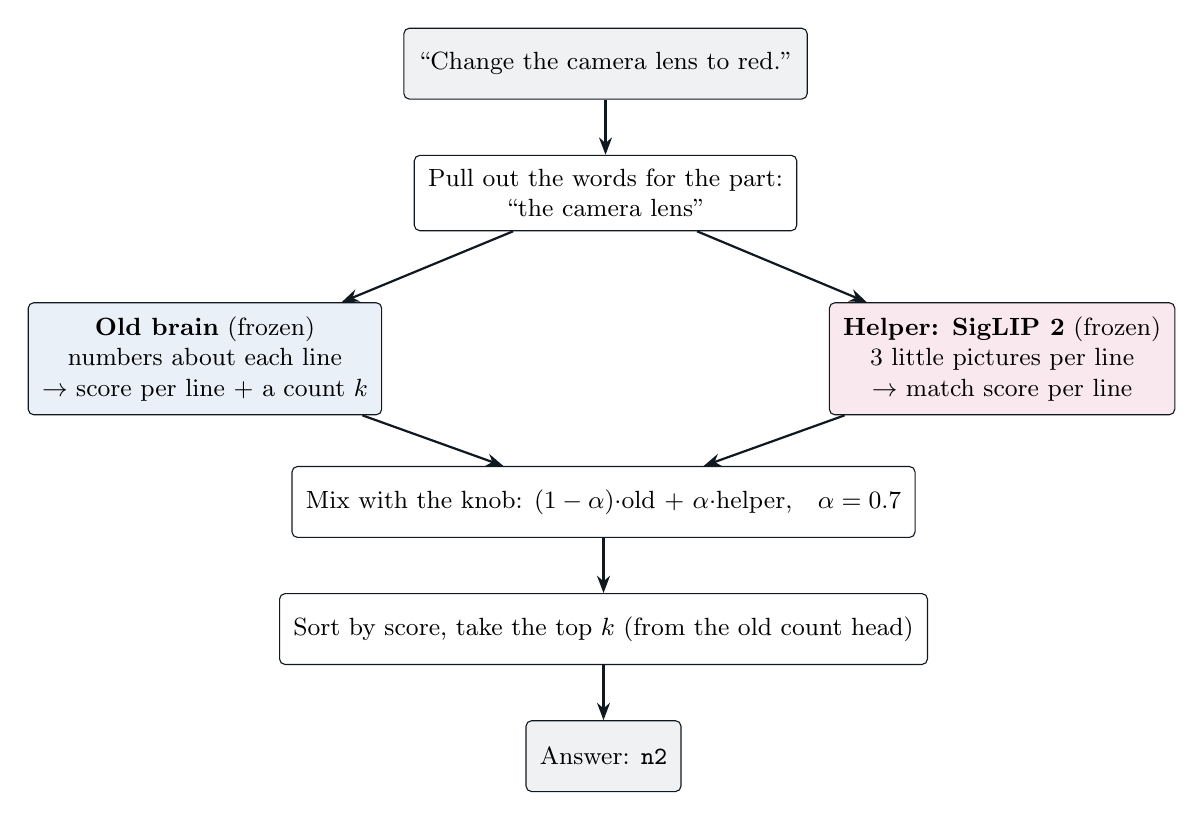
\begin{tikzpicture}[
  node distance=7mm and 9mm,
  box/.style={draw=ink, rounded corners=2pt, align=center, font=\small, inner sep=5pt, minimum height=9mm},
  arrow/.style={-{Stealth[length=2.2mm]}, line width=0.8pt, ink}
]
  \node[box, fill=grey!12] (instr) {``Change the camera lens to red.''};
  \node[box, below=of instr] (phrase) {Pull out the words for the part:\\``the camera lens''};
  \node[box, below left=9mm and 4mm of phrase, fill=blue!10] (mlp) {\textbf{Old brain} (frozen)\\numbers about each line\\$\to$ score per line + a count $k$};
  \node[box, below right=9mm and 4mm of phrase, fill=pink!10] (sig) {\textbf{Helper: SigLIP 2} (frozen)\\3 little pictures per line\\$\to$ match score per line};
  \node[box] (mix) at ($(mlp.south)!0.5!(sig.south) + (0,-11mm)$) {Mix with the knob: $(1-\alpha)\cdot$old $+\ \alpha\cdot$helper,\quad $\alpha = 0.7$};
  \node[box, below=of mix] (pick) {Sort by score, take the top $k$ (from the old count head)};
  \node[box, below=of pick, fill=grey!12] (ans) {Answer: \texttt{n2}};
  \draw[arrow] (instr) -- (phrase);
  \draw[arrow] (phrase) -- (mlp);
  \draw[arrow] (phrase) -- (sig);
  \draw[arrow] (mlp) -- (mix);
  \draw[arrow] (sig) -- (mix);
  \draw[arrow] (mix) -- (pick);
  \draw[arrow] (pick) -- (ans);
\end{tikzpicture}
\end{center}

\needspace{14\baselineskip}
\section*{What happened}

We ran the real test once. Here is what each version of the machine got exactly right.

\begin{center}
\small
\begin{tabular}{@{}lrrrr@{}}
\toprule
Version & Right / 100 & One-line / 55 & Many-line / 45 & Wrong part \\
\midrule
Old brain (the baseline) & 22 & 18 & 4 & 48 \\
Trained top-$k$ head (yesterday's best) & 27 & 23 & 4 & 50 \\
Helper only ($\alpha = 1$) & 37 & 36 & 1 & 26 \\
\textbf{Old brain + helper ($\alpha = 0.7$)} & \textbf{39} & 35 & 4 & 28 \\
\bottomrule
\end{tabular}
\end{center}

In plain words:
\begin{itemize}[leftmargin=1.6em]
  \item The mix went from 22 to \textbf{39} right answers. That is 17 more. Even after allowing for luck (a statistical check that shuffles the icons 5{,}000 times), the gain is somewhere between 10 and 24. It is real.
  \item It beat yesterday's best system, which had actually been \emph{trained}, by 12. Today's addition was not trained at all.
  \item Wrong-part mistakes fell from 48 to 28.
  \item It fixed 19 drawings and broke 2. The 19 were all about words: bolt, bell, hull, antenna, chestpiece. The 2 it broke were tiny marks described by position (``the small dot below the arcs''), where the old brain had been right.
  \item Helper-only got 37, almost as good, but it loses the many-line answers (1 instead of 4). Mixing keeps them.
\end{itemize}

\section*{What is still broken: counting}

Look at the ``many-line answers'' column: \textbf{4 out of 45}, for every version.
The mix did not touch it, because we only changed the \emph{order} of the lines, not \emph{how many} are picked.

The count head almost always says ``one''. It said ``one'' in \textbf{71 of the 100} drawings, even though only 55 needed one line.
For ``both truck wheels'' the mix put the two wheels first, and then the count head said ``four'', so it also grabbed the cab and the box.
For ``all three paint wells'' it put the three wells first and the count head said ``one''.

If the count were right, the mix would get \textbf{60 out of 100}. That is the prize for the next experiment.

We tried a few simple counting fixes on the \emph{practice exam}: pick every line whose score is close to the best one, or use the count head's average guess.
The best gained only 3 drawings out of 80.
We did \textbf{not} try them on the real test, and we did not invent a rule from the real test's sentences, because that would be peeking at the answers.

\section*{How we kept it fair}

\begin{itemize}[leftmargin=1.6em]
  \item The real test is sealed with a fingerprint. The old brain is sealed the same way.
  \item The only knob was chosen on the practice exam with a rule written down first, then frozen in git before the real test ran.
  \item The helper's own settings (which three pictures, how to mix them) came from an earlier experiment and were not touched.
  \item Before designing the mix, I had looked at 14 of the 100 real-test drawings while studying the old mistakes. I did not change anything after that. This is written in the report so a reader can discount it.
  \item The real test has now been scored three times in total (twice yesterday for a different experiment, once today). The report says so.
  \item The right answers were written and checked by the agent, not by outside people. The drawings are line icons. The result may not carry to messy real-world clip art.
\end{itemize}

\section*{What it costs}

The old brain takes about 5 milliseconds per drawing.
With the helper it takes about 300 milliseconds on a laptop GPU, because it has to draw three little pictures per line and run a big model on them.
The helper is a 1.4~GB download.
So it is about 60 times slower and much heavier, in exchange for almost twice as many right answers.

\section*{What comes next}

Fix the counting. That needs a fair way to learn ``how many lines'', tested on drawings that are neither the sealed real test nor the rough practice exam: a new small set of icons with hand-written counts, or practice instructions that say ``both'' and ``all three''.
Keep today's mix, the old brain, and the 100 sealed answers exactly as they are, and run it once.

\section*{Where the files are}

Everything is on the git branch \texttt{agent/svg-group-candidate-v6} of \href{https://github.com/ayushdebnath012/SVG}{\texttt{ayushdebnath012/SVG}}.
\begin{itemize}[leftmargin=1.6em]
  \item The full write-up with all the numbers: \texttt{docs/SEMANTIC\_PRIOR\_RESULTS.md}.
  \item The frozen knob and fingerprints: \texttt{configs/eval/semantic\_prior\_v1.json}.
  \item The program: \texttt{scripts/run\_semantic\_prior\_grounding.py}.
  \item Every score for every line in every drawing: \texttt{runs/semantic-prior-v1/records.json}.
  \item The sealed real test: \texttt{data/group-holdout-v1/}.
\end{itemize}

\end{document}
